\documentclass{standalone}

\begin{document}

\subsection[U-Net model]{U-Net model}\label{segmentation:Unet}

U-Net neural network model is one of the state-of-art model in image segmentation.
It was firstly developed for biomedical image segmentation but it showed its efficiency also in different application tasks and different research topics.
Its backbone is intrinsically a \quotes{common} CNN but the structure can be divided into two macro paths.
The first path of the model is a contraction path (or \emph{encoder}) while the second path is an expansion path (or \emph{decoder}).
The first set of layers in the model, in fact, are a sequence of convolutional and pooling layers which aim to extract features and reduce the dimensionality of the input in the same way as an encoder convert a signal to a smaller range of values.
The extracted features are then processed by the decoder, i.e a second set of convolutional and up-sampling layers, to reconstruct the feature map size and the segmentation mask.
An illustrative representation of the model structure is provided in Fig.~\ref{fig:unet}.

\begin{center}
\begin{figure}[htbp]
\centering
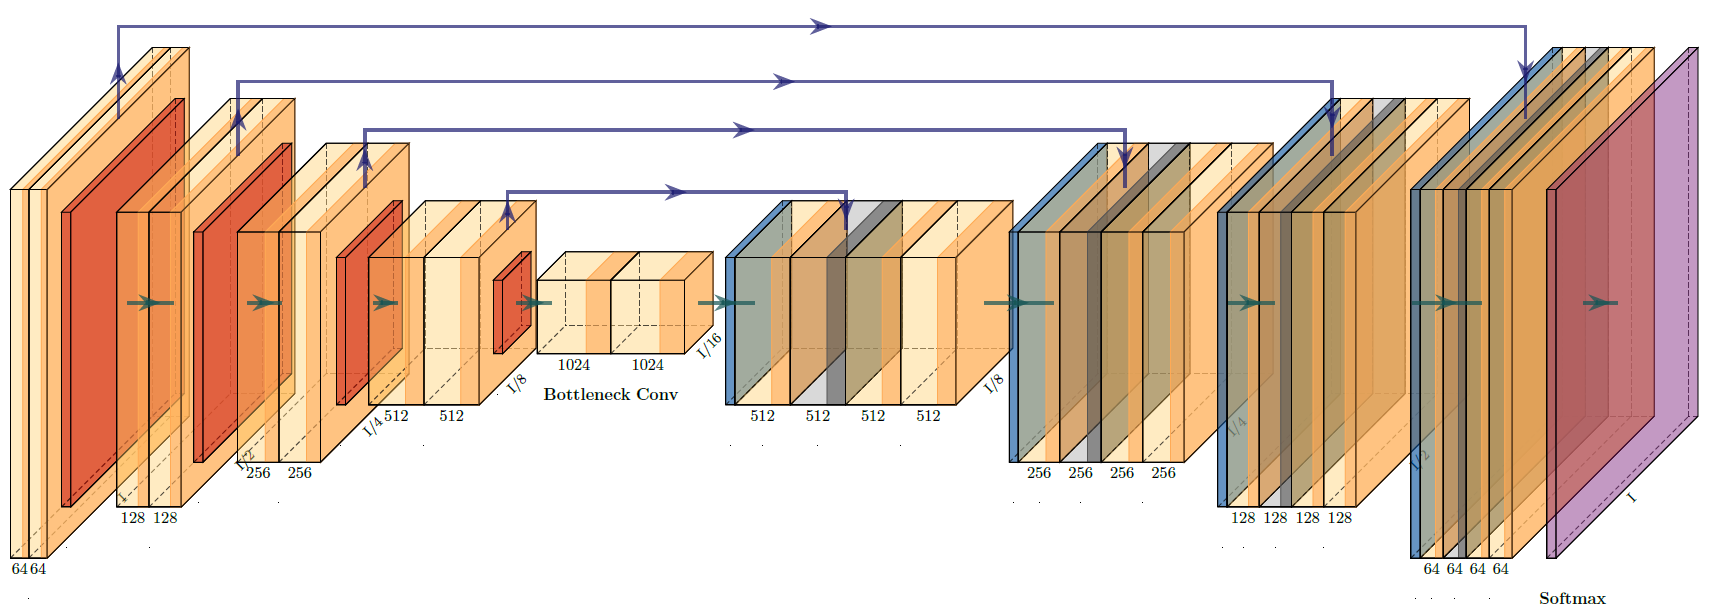
\includegraphics[width=0.85\textwidth]{unet.png}
\caption{U-Net model scheme.
The first part of the structure represents the encoder while the tail of the model is the decoder part.
The model name is given by the numerous shortcut connections which link the encoder layers to the decoder ones: if we contract the long-range connections the global structure acquire a U form.
The figure was generated using the \href{https://github.com/HarisIqbal88/PlotNeuralNet}{PlotNeuralNet} package of H. Iqbal.
}
\label{fig:unet}
\end{figure}
\end{center}

We have already discussed about the functionality of each layers in the previous sections and also in this kind of model a key role was performed by the shortcut connections.
The decoding path tends to lose some of the higher level features the encoder learned: using shortcut connections the output of the encoding layers are passed directly to the decoding layers so that all the important pieces of information can be preserved.

In the previous sections we have also described the common loss functions used to train Neural Network models.
Considering the \quotes{simple} segmentation of an object from its background, the ground truth mask, i.e the \quotes{label} of the input image, would be a binary matrix.
In these cases a valid loss function (also used in our applications) could be the \emph{binary cross-entropy} (ref. \ref{NN:cost}).

\begin{center}
\begin{figure}[htbp]
\centering
\def\svgwidth{0.85\textwidth}
\input{./img/iou_example.pdf_tex}
\caption{IoU score example.
The IoU score is computed as the area intersection of the two boxes over their union.
Starting from the left we can see an increment of the overlap between the two boxes related to an increment in their IoU scores.
}
\label{fig:iou_example}
\end{figure}
\end{center}

A word of caution must be spent about the metrics to evaluate the performances of our model.
Standard metrics, as the \emph{accuracy}\footnote{
  The accuracy measures the number of true positives + false negatives outputs on the total number of predictions.
}, are not good measures to face on the segmentation problem.
If we want to identify and segment an object into an image we can reasonably assume that the number of pixels concerning the object would be very few against the number of pixels related to the background.
Thus the told above binary mask would be a matrix with a large amount of zeros and only few ones.
In this case the standard metric functions have to consider an unbalanced number of samples: if the model outputs a matrix of all zeros the accuracy of it will be high despite the informative values are only the few pixel equals to one.
A possible solution to overcome this problem is given by the \emph{mean IoU score} which measures the average IoU between the output mask and the binary ground truth:

$$
\mbox{IoU} = \frac{\mbox{Area of Overlap}}{\mbox{Area of Union}}
$$

The efficiency and meaning of this score can be visible in Fig.~\ref{fig:iou_example}.

\end{document}
